%%%%%%%%%%%%%%%%%%%%%%%%%%%%%%%%%%%%%%%%%
% Cleese Assignment (For Students)
% LaTeX Template
% Version 2.0 (27/5/2018)
%
% This template originates from:
% http://www.LaTeXTemplates.com
%
% Author:
% Vel (vel@LaTeXTemplates.com)
%
% License:
% CC BY-NC-SA 3.0 (http://creativecommons.org/licenses/by-nc-sa/3.0/)
% 
%%%%%%%%%%%%%%%%%%%%%%%%%%%%%%%%%%%%%%%%%

%----------------------------------------------------------------------------------------
%	PACKAGES AND OTHER DOCUMENT CONFIGURATIONS
%----------------------------------------------------------------------------------------

\documentclass[fleqn]{article}
\usepackage{listings}
\usepackage{color} %red, green, blue, yellow, cyan, magenta, black, white
\definecolor{mygreen}{RGB}{28,172,0} % color values Red, Green, Blue
\definecolor{mylilas}{RGB}{170,55,241}
\usepackage{amsmath, amssymb}
\DeclareMathOperator{\sinc}{sinc}
\DeclareMathOperator{\sgn}{sgn}

\input{structure.tex} % Include the file specifying the document structure and custom commands

%----------------------------------------------------------------------------------------
%	ASSIGNMENT INFORMATION
%----------------------------------------------------------------------------------------

% Required
\newcommand{\assignmentQuestionName}{Question} % The word to be used as a prefix to question numbers; example alternatives: Problem, Exercise
\newcommand{\assignmentClass}{Communication Systems (Taught by Mohammad Hadi)\\Assignment 3 (Due on DDD.,\ mmm.\ dd,\ yyyy)} % Course (Lecturer)\\Assignment (Due date)
\newcommand{\assignmentTitle}{} % Assignment title or name
\newcommand{\assignmentAuthorName}{Radin khayyam\\99101579} % Student name\\Student number
%----------------------------------------------------------------------------------------

\begin{document}
\lstset{language=Matlab,%
    basicstyle={\scriptsize},
    breaklines=true,%
    morekeywords={matlab2tikz},
    keywordstyle=\color{blue},%
    morekeywords=[2]{1}, keywordstyle=[2]{\color{black}},
    identifierstyle=\color{black},%
    stringstyle=\color{mylilas},
    commentstyle=\color{mygreen},%
    showstringspaces=false,%without this there will be a symbol in the places where there is a space
    numbers=left,%
    numberstyle={\tiny \color{black}},% size of the numbers
    numbersep=5pt, % this defines how far the numbers are from the text
    emph=[1]{break},emphstyle=[1]\color{red}, %some words to emphasise
    %emph=[2]{word1,word2}, emphstyle=[2]{style},    
}
%----------------------------------------------------------------------------------------
%	TITLE PAGE
%----------------------------------------------------------------------------------------

\assignmentSection{Mathematical Questions}
%----------------------------------------------------------------------------------------
%	QUESTION 1
%----------------------------------------------------------------------------------------

\begin{question}
\questiontext{A vestigial-sideband modulation system is depicted in Fig. \ref{fig:Q1}. The bandwidth of the message signal $m(t)$ is $W$, and the transfer function of the bandpass filter is shown in the figure.}
\begin{figure}[h]
\centering
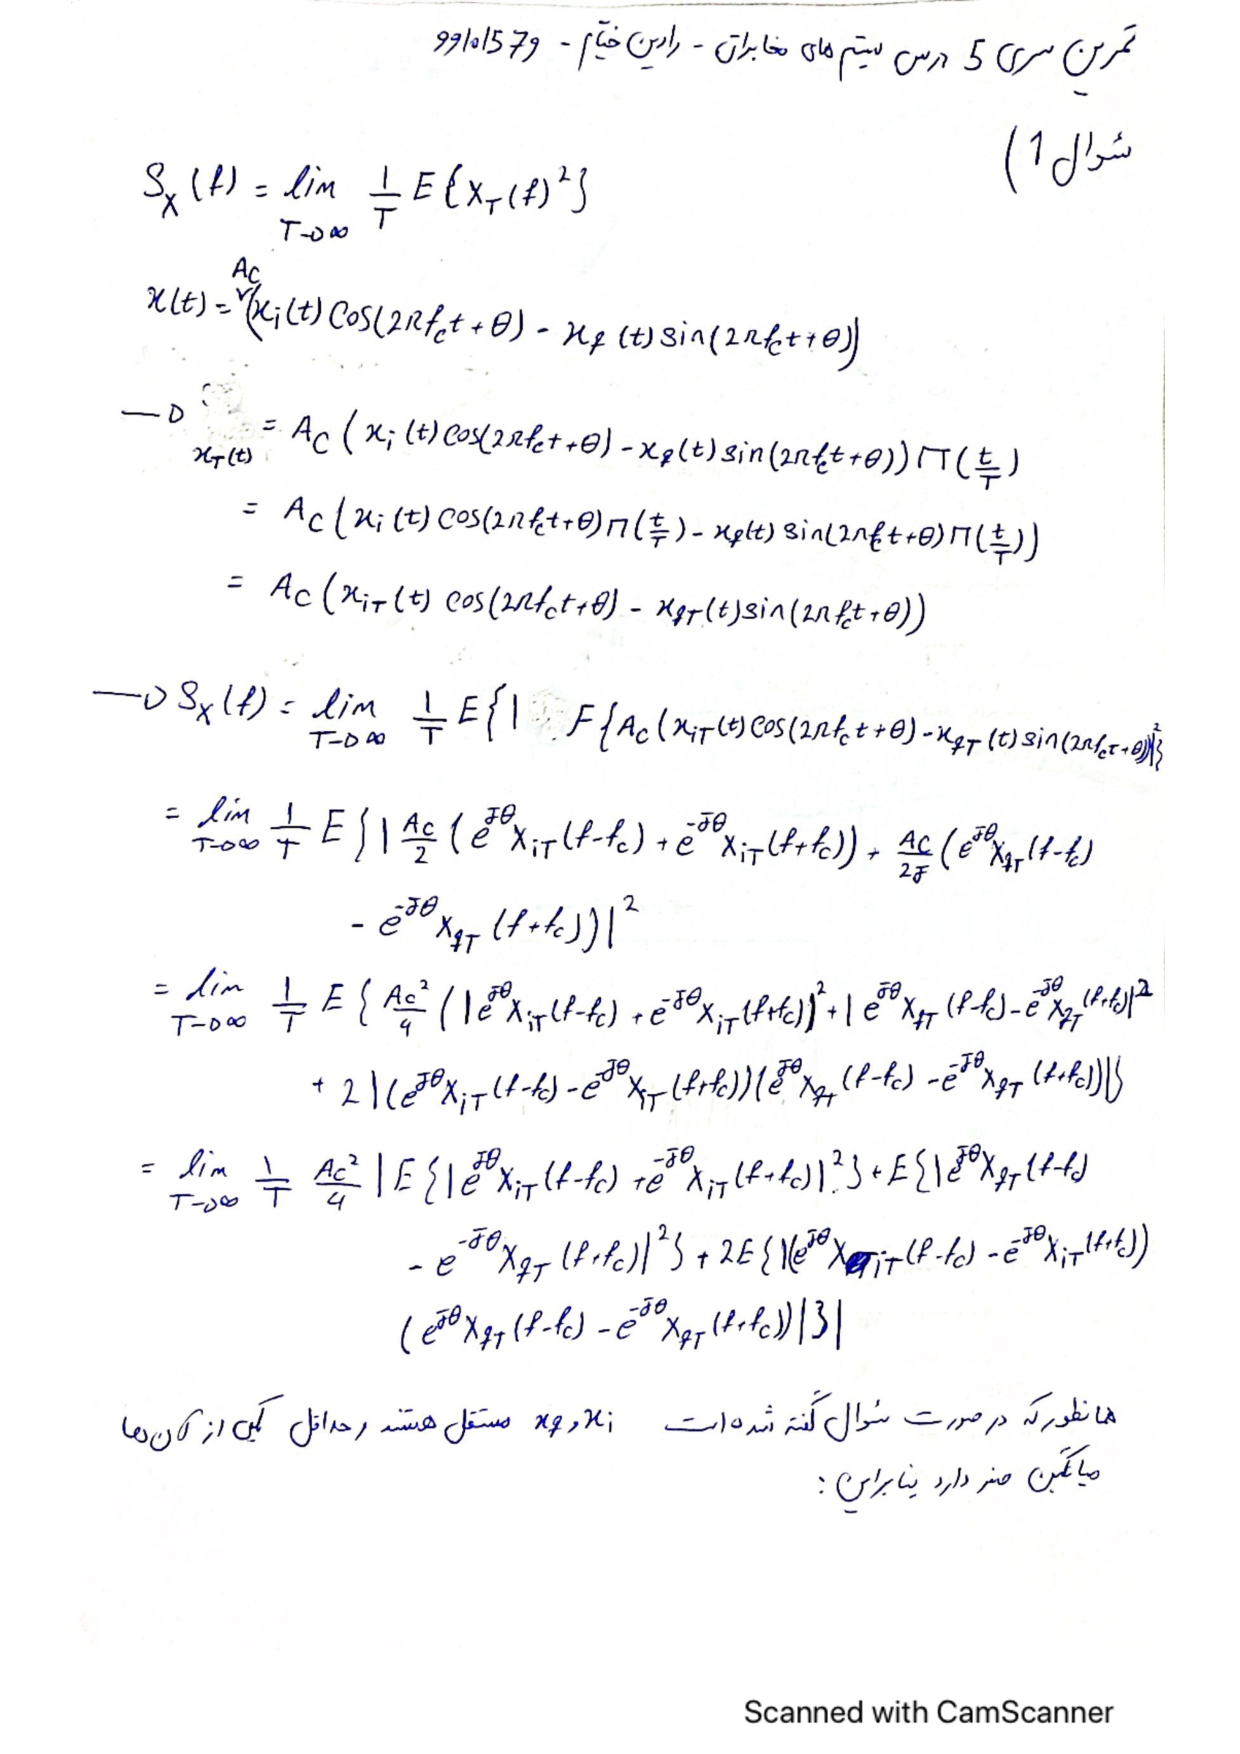
\includegraphics[scale=0.75]{Fig/Q1.pdf}
\caption{A VSB modulation system.}\label{fig:Q1}
\end{figure}

%--------------------------------------------
\begin{subquestion}{Determine $h_l(t)$, the lowpass equivalent of $h(t)$, where $h(t)$ represents the impulse response of the bandpass filter.
}\label{Q1a}
\answer{
\[ H_{l}(f) = 2H(f+f_{c})u(f+f_{c}) \rightarrow
     H_{l}(f)=\left\{
                \begin{array}{ll}
                  \frac{-2}{W}f+1, \hspace{1cm}|f|\leq \frac{W}{2} \\~\\
                  2, \hspace{2cm}-W \leq f  < \frac{-W}{2}
                \end{array}
              \right.
\]
\[ h(t) = \mathcal{F}^{-1}\{ H_{l}(f) \} = \int_{-\infty}^{+\infty} H_{l}(f)e^{j2\pi ft} \,df = \int_{-\frac{W}{2}}^{+\frac{W}{2}}(\frac{-2}{W}f+1)e^{j2\pi ft}\, df + \int_{-W}^{\frac{-W}{2}}2e^{j2\pi ft}\,df \]
\[= \frac{-2}{W}\left(\frac{1}{j2\pi t}fe^{j2\pi ft}-\frac{1}{(j2\pi t)^2}e^{j2\pi ft}\right)\bigg \rvert_{\frac{-W}{2}}^{\frac{W}{2}} +\left(\frac{1}{j2\pi t}e^{j2\pi ft}\right)\bigg \rvert_{\frac{-W}{2}}^{\frac{W}{2}} + \left(\frac{2}{j2\pi t}e^{j2\pi ft}\right)\bigg \rvert_{-W}^{\frac{-W}{2}} \]
\[= \left(\frac{-1}{j2\pi t}\left(e^{j\pi Wt}+e^{-j\pi Wt}\right)+\frac{-2}{4\pi^{2}t^{2}W}\left(e^{j\pi Wt}-e^{-j\pi Wt}\right)\right) +\frac{1}{j2\pi t}\left(e^{j\pi Wt}-e^{-j\pi Wt}\right)\]
\[  + \frac{1}{j\pi t}\left(e^{-j\pi Wt}-e^{-j2\pi Wt}\right) \] 
\[ = \frac{1}{j\pi t}e^{-j2\pi Wt} - \frac{j}{\pi^{2}t^{2}W}\sin(\pi Wt) = \boxed{\frac{1}{j\pi t}\left(e^{-j2\pi Wt}+\sinc(Wt)\right)}\]
}
\end{subquestion}

%--------------------------------------------
\begin{subquestion}{Derive an expression for the modulated signal $u(t)$.
} 
\answer{
\[u(t) = A_{c}m(t)\cos(2\pi f_{c}t) * h(t) = A_{c}m(t) \mathcal{R}\{ e^{j2\pi f_{c}t }\}  * h(t)\]
\[  h(t)=\mathcal{R}\{ x_{l}(t)e^{j2\pi f_{c} t} \} \rightarrow u(t) = A_{c}m(t) \mathcal{R}\{ e^{j2\pi f_{c}t }\} *\mathcal{R}\{ e^{j2\pi f_{c}t }\}   \]
\[\rightarrow u(t) = \mathcal{R} \{ A_{c}m(t) * h_{l}(t)  \}e^{j2\pi f_{c}t}   \]
\[\rightarrow u(t) = \mathcal{R} \{ A_{c}m(t) * \frac{1}{j\pi t}(e^{-j2\pi Wt}+\sinc(Wt))  \}e^{j2\pi f_{c}t}   \]
\[ = \mathcal{R}\{ (A_{c}m(t)*\frac{1}{j\pi t}\sinc(Wt))e^{j2\pi f_{c}t} - (A_{c}m(t)*\frac{1}{j\pi t}e^{-j2\pi Wt})e^{j2\pi f_{c}t}\} \]
\[ \mathcal{F} \{ m(t) * \frac{1}{j\pi t}e^{-j2\pi Wt}\}=-M(f)sgn(f+W)=-M(f) \rightarrow m(t)*\frac{1}{j\pi t} e^{-j2\pi Wt}  = -m(t) \]
\[ \rightarrow u(t)=\mathcal{R}\{(A_{c} m(t)*(\frac{1}{j\pi t}\sinc(Wt)))e^{j 2\pi f_{c}t} - A_{c}m(t)e^{-j2\pi f_{c}t} \}  \]
\[\rightarrow \boxed{ u(t)=-A_{c}m(t)cos(2\pi f_{c}t) -A_{c}(m(t)*\frac{1}{\pi t}\sinc(Wt))\sin(2\pi f_{c}t )} \]
}
\end{subquestion}
\end{question}

%----------------------------------------------------------------------------------------
%	QUESTION 2
%----------------------------------------------------------------------------------------

\begin{question}

\questiontext{Follow the steps below to show the power of the FM signal $u(t)=A_c\cos(2\pi f_ct+\phi(t))$ is $\frac{A_c^2}{2}$.
}
%--------------------------------------------
\begin{subquestion}{Write the power expression for the FM
signal and show that the power equals $P=\frac{A_c^2}{2}+I
$, where
$$
I=\lim_{T\rightarrow \infty} \frac{A_c^2}{2T}\int_{-T/2}^{T/2} \cos(4\pi f_c t +2\phi(t))dt
$$
} 
\answer{
\[P = \lim_{T\rightarrow \infty} \frac{1}{T} \int_{-T/2}^{T/2} u^2 (t) dt = \frac{1}{T} \int_{-T/2}^{T/2} A_c^2 \cos^2 (2\pi f_c t + \phi(t)) dt \]
\[= \frac{A_c^2}{2} +  \lim_{T\rightarrow \infty} \frac{A_c^2}{2T}\int_{-T/2}^{T/2} \cos(4\pi f_c t +2\phi(t))dt = \frac{A_c^2}{2}+I \]
\[\rightarrow \boxed{I=\lim_{T\rightarrow \infty} \frac{A_c^2}{2T}\int_{-T/2}^{T/2} \cos(4\pi f_c t +2\phi(t))dt} \]
}
\end{subquestion}
%--------------------------------------------
\begin{subquestion}{
Show that 
$$
I_{\infty}=\int_{-\infty}^\infty \cos(4\pi f_c t +2\phi(t))dt
$$
relates to the Fourier transforms $\mathcal{F}\{e^{j2\phi(t)}\}$ and $\mathcal{F}\{e^{-j2\phi(t)}\}$ at the frequencies $-2f_c$ and $2f_c$, respectively. 
}
\answer{
\[I_{\infty}=\int_{-\infty}^\infty \cos(4\pi f_c t +2\phi(t))dt = \int_{-\infty}^\infty \frac{1}{2}(e^{(j 4\pi f_c t +2\phi(t))} + e^{(-j 4\pi f_c t +2\phi(t))}) dt\]
\[ = \int_{-\infty}^\infty \frac{1}{2} (e^{4\pi f_c t} \times e^{2j \phi(t)}) + \int_{-\infty}^\infty \frac{1}{2} (e^{-4\pi f_c t} \times e^{-2j \phi(t)})\]
\[=\boxed{ \frac{1}{2} \mathcal{F}\{e^{j2\phi(t)}\}|_{f=-2f_c} + \frac{1}{2} \mathcal{F}\{e^{-j2\phi(t)}\}|_{f=2f_c}}\]

}
\end{subquestion}
%--------------------------------------------
\begin{subquestion}{Use Taylor series expansion to show that $I_{\infty}$ depends to the Fourier transforms $\mathcal{F}\{\phi^n(t)\}, n \in \mathbb{W}$ at the frequency $\pm 2f_c$.
}
\answer{
\[I_{\infty} = \frac{1}{2} \mathcal{F}\{1 + 2j\phi(t) + \frac{(2j\phi(t))^2}{2!} +
\frac{(2j\phi(t))^3}{3!} + ... \}|_{f=-2f_c} \]
\[+ \frac{1}{2} \mathcal{F}\{1 - 2j\phi(t) + \frac{(2j\phi(t))^2}{2!} -
\frac{(2j\phi(t))^3}{3!} + ... \}|_{f=2f_c} \]
\[= \boxed{\frac{1}{2} \sum_{n=0}^{\infty} \frac{(2j)^n}{n!} \mathcal{F}\{ \phi^n (t) \}|_{f=-2f_c} + \frac{1}{2} \sum_{n=0}^{\infty} \frac{(-2j)^n}{n!} \mathcal{F}\{ \phi^n (t) \}|_{f=2f_c}}\]
}
\end{subquestion}
%--------------------------------------------
\begin{subquestion}{Show that if $f_c\gg W$, where $W$ is the bandwidth of the message-related phase $\phi(t)$, $I_{\infty}\approx 0$. 
}
\answer{

}
\end{subquestion}
%--------------------------------------------
\begin{subquestion}{Show that the power is approximately equal to $\frac{A_c^2}{2}$. 
}
\answer{}
\end{subquestion}
\end{question}
\pagebreak
%----------------------------------------------------------------------------------------
%	QUESTION 3
%----------------------------------------------------------------------------------------

\begin{question}
\questiontext{Find the spectrum of the narrowband FM signal $$
u(t)=A_c\cos(2\pi f_c t)-A_c\big[2\pi k_f \int_{-\infty}^tm(\tau)d\tau\big]\sin(2\pi f_c t)
$$ 
and narrowband PM signal
$$
u(t)=A_c\cos(2\pi f_c t)-A_ck_pm(t)\sin(2\pi f_c t)
$$ 
in terms of the message spectrum $M(f)$.
}

\answer{
\[u(t)=A_c\cos(2\pi f_c t)-A_c\big[2\pi k_f \int_{-\infty}^tm(\tau)d\tau\big]\sin(2\pi f_c t)  \]
\[ \rightarrow U(f) = \mathcal{F}\{A_c\cos(2\pi f_c t) \}-\mathcal{F}\{ 2\pi k_f \int_{-\infty}^tm(\tau)d\tau \} * \mathcal{F}\{A_{c}\sin(2\pi f_{c}t)\} \]
\[\mathcal{F}\left\{\int_{-\infty}^t m(\tau)d\tau\right\} = \frac{M(f)}{2j \pi f} + \frac{1}{2} M(0) \delta(f) \]
\[\rightarrow  U(f) = \frac{A_c}{2}[\delta(f-f_c) + \delta(f+ f_c)] - \frac{2A_c\pi k_f}{2j}[\delta(f - f_c) - \delta(f + f_c)] * [\frac{M(f)}{2j\pi f} + \frac{M(0)\delta(f)}{2}]  \]
\[=\frac{A_c}{2}[\delta(f-f_c) + \delta(f+ f_c)] + 2A_c \pi k_f [\frac{M(f-f_c)}{4\pi (f-f_c)} - \frac{ M(f+f_c)}{4\pi (f+f_c)} +\frac{j  M(0) \delta(f-f_c)}{4}\]
\[- \frac{j  M(0) \delta(f+f_c)}{4}]  \]
if assume M(0)=0,
\[\rightarrow \boxed{U_{f}=\frac{A_c}{2}[\delta(f-f_c) + \delta(f+ f_c)] +\frac{A_c kf}{2} [\frac{M(f-f_c)}{(f-f_c)} - \frac{ M(f+f_c)}{(f+f_c)}]} \]
}

\end{question}

%----------------------------------------------------------------------------------------
%	QUESTION 4
%----------------------------------------------------------------------------------------

\begin{question}
\questiontext{The cross-correlation of the power signals $w(t)$ and $v(t)$ is defined as $R_{vw}(\tau)=\langle v(t)w^*(t-\tau)\rangle$, where the time average operator $$\langle x(t)\rangle=\lim_{T\rightarrow \infty} \frac{1}{T}\int_{-T/2}^{T/2} x(t)dt$$.}

%--------------------------------------------
\begin{subquestion}{Show that $R_{vw}(\tau)=R^*_{wv}(-\tau)$.
} 
\answer{
we can obtain that,
\[\langle x(t) \rangle^* = [\lim_{T\rightarrow \infty}\int_{-T/2}^{T/2} x(t) dt]^* = \lim_{T\rightarrow \infty}\int_{-T/2}^{T/2} x^*(t) dt = \langle x^*(t) \rangle\]
so we will have,
\[ R^*_{wv}(-\tau)=[\langle w(t) v^*(t+\tau) \rangle ]^* = \langle w^*(t) v(t+\tau) \rangle = \lim_{T\rightarrow \infty}\int_{-T/2}^{T/2} w^*(t) v(t+\tau) dt  \] \[  t=t-\tau \rightarrow R^*_{wv}(-\tau)=\lim_{T\rightarrow \infty}\int_{-T/2 - \tau}^{T/2 -\tau} w^*(t-\tau) v(t) dt = \lim_{T\rightarrow \infty}\int_{-T/2}^{T/2} w^*(t-\tau) v(t) dt \]
\[ \rightarrow \boxed{R_{vw}(\tau)=R_{wv}^{*}(-\tau)}\]
}
\end{subquestion}

%--------------------------------------------
\begin{subquestion}{Prove that $|R_{vw}(\tau)|^2 \leqslant P_v P_w$.
} 
\answer{}
\end{subquestion}
\end{question}

%----------------------------------------------------------------------------------------
%	QUESTION 5
%----------------------------------------------------------------------------------------

\begin{question}

\questiontext{Fig. \ref{fig:Q5} shows the block diagram of an FM to AM demodulator and the schematic of its practical implementation, which is called balanced FM demodulator or FM discriminator. }
\begin{figure}[h]
\centering
\includegraphics[scale=0.45]{Fig/Q5.png}
\caption{Balanced FM demodulator.}\label{fig:Q5}
\end{figure}
%--------------------------------------------
\begin{subquestion}{Find the output of the FM to AM converter block if its frequency response is $H(f)=j[V_0+k(f-f_c), \quad |f-f_c|<0.5B_c$, where $B_c$ denotes the bandwidth of the input FM modulated signal $u(t)=A_c\cos(2\pi f_c t +2\pi k_f \int_{-\infty}^t m(\tau)d\tau)$. Note that the FM to AM impulse response is real and therefore, $H(-f)=H^*(f)$.
} 
\answer{

}
\end{subquestion}

%--------------------------------------------
\begin{subquestion}{Explain how the shown schematic implements the FM to AM demodulator? Why are there two filters and two envelope detectors in the schematic?
} 
\answer{}
\end{subquestion}

\end{question}

%----------------------------------------------------------------------------------------

\assignmentSection{Software Questions}

%----------------------------------------------------------------------------------------
%	QUESTION 6
%----------------------------------------------------------------------------------------
\begin{question}

\questiontext{Develop a MATLAB/Python code that plots the cross-correlation $R_{vw}(\tau)$ of two power signals $v(t)$ and $w(t)$. Illustrate the output of the code for sample power signals.  
}

\answer{}
\end{question}

%----------------------------------------------------------------------------------------

\assignmentSection{Bonus Questions}

%----------------------------------------------------------------------------------------
%	QUESTION 7
%----------------------------------------------------------------------------------------

\begin{question}

\questiontext{Two power signals of $v(t)$ and $w(t)$ are called uncorrelated if their cross-correlation $R_{vw}(\tau)=0, \forall \tau$. Show that for these uncorrelated signals, the power $P_z$ of $z(t)=v(t)+w(t)$ equals $P_z=P_v+P_w$.}

\answer{
\[
P_z = \lim_{T\rightarrow \infty} \frac{1}{T}\int_{-T/2}^{T/2} |z|^2 dt = \lim_{T\rightarrow \infty} \frac{1}{T}\int_{-T/2}^{T/2} z z^* dt = \lim_{T\rightarrow \infty} \frac{1}{T}\int_{-T/2}^{T/2} (v + w)(v^* + w^*) dt\]
\[ = \lim_{T\rightarrow \infty} \frac{1}{T}\int_{-T/2}^{T/2} |v|^2 dt + \lim_{T\rightarrow \infty} \frac{1}{T}\int_{-T/2}^{T/2} |w|^2 dt + \lim_{T\rightarrow \infty} \frac{1}{T}\int_{-T/2}^{T/2} v(t) w^*(t) dt \]
\[+ \lim_{T\rightarrow \infty} \frac{1}{T}\int_{-T/2}^{T/2} v^*(t) w(t) dt \]
\[= \boxed{P_v + P_w + \lim_{T\rightarrow \infty} \frac{1}{T}\int_{-T/2}^{T/2} v(t)w^*(t) dt + \lim_{T\rightarrow \infty} \frac{1}{T}\int_{-T/2}^{T/2} v^*(t)w(t) dt}\]
\[R_{vw}(\tau)= \lim_{T\rightarrow \infty} \frac{1}{T}\int_{-T/2}^{T/2} v(t)w^*(t-\tau) dt =0\]
\[ \rightarrow R_{vw}(0) = \lim_{T\rightarrow \infty} \frac{1}{T}\int_{-T/2}^{T/2} v(t)w^*(t) = 0\]
 \[ \rightarrow R_{vw}^*(\tau) = 0 \rightarrow \lim_{T\rightarrow \infty} \frac{1}{T}\int_{-T/2}^{T/2} v^*(t)w(t) = 0\]
\[\boxed{\rightarrow P_z = P_v + P_w}\]
}

\end{question}


%----------------------------------------------------------------------------------------
%	QUESTION 7
%----------------------------------------------------------------------------------------

\begin{question}

\questiontext{Return your answers by filling the \LaTeX template of the assignment.}

\end{question}

%----------------------------------------------------------------------------------------

\end{document}
